\begin{figure*}[t]
\centering
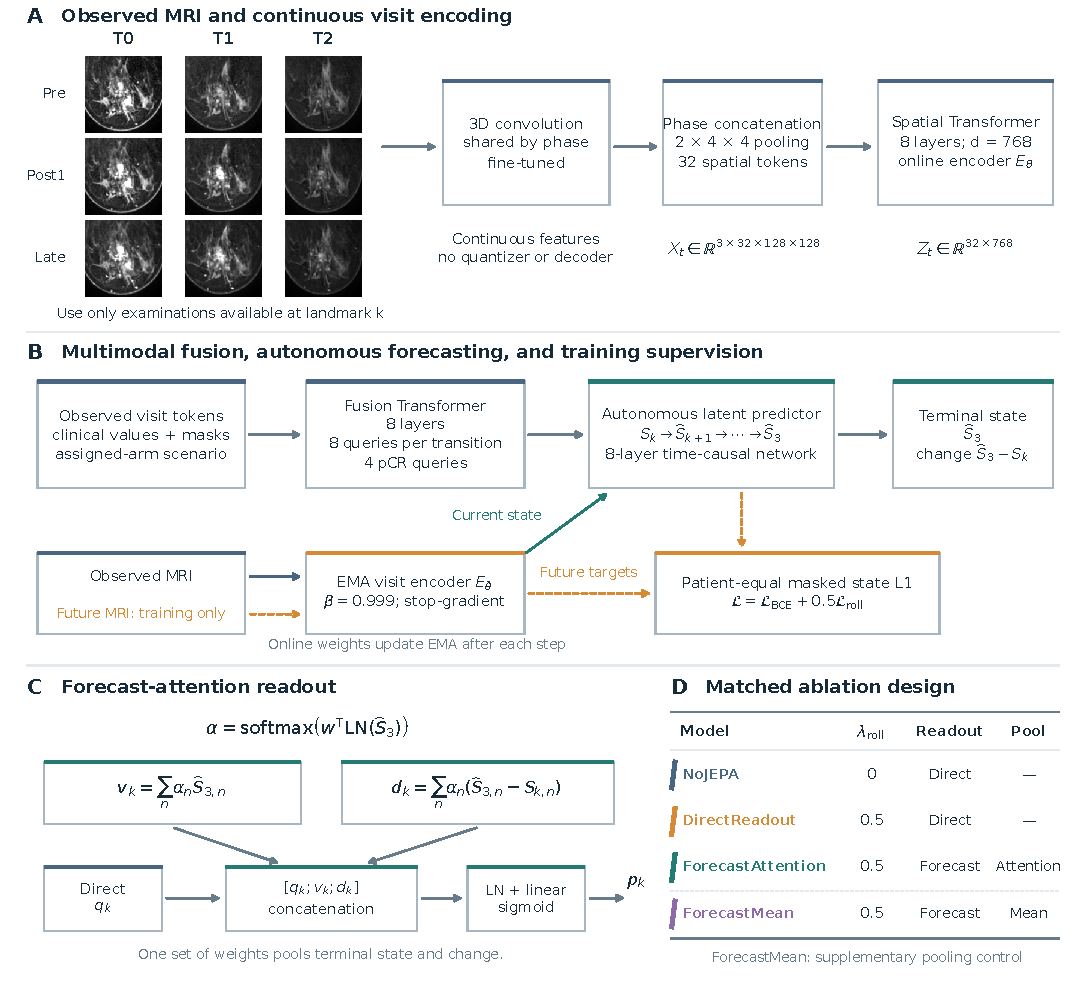
\includegraphics[width=\textwidth]{figures/framework.pdf}
\caption{Forecast-aware latent modeling and matched controls. (A) Real three-phase MRI crops from one development patient illustrate the same baseline-defined plane at T0, T1, and T2; the example and slice were selected without outcomes or pCR predictions. Only visits available at the prediction landmark are inputs. A shared continuous encoder and spatial Transformer produce visit tokens. (B) Clinical values, availability masks, and an assigned-arm scenario condition fusion and autonomous prediction to T3. The EMA encoder supplies the detached current state; available future MRI supplies training targets only. Dashed orange arrows denote training-target or loss paths. (C) Attention weights pool the predicted terminal state and its change; these features are combined with direct pCR-query features. (D) The primary variants separate removal of future-state supervision from the complete forecast readout. ForecastMean is a supplementary pooling control. One fold model is illustrated. Within each of seeds 42, 44, 2026, and 3407, evaluation averages five fold probabilities per patient before computing metrics; reported performance then averages the four seed metrics, without ensembling probabilities across seeds. MRI tiles are illustrative crops, not generated images, segmentation ground truth, or attention maps.}
\label{fig:framework}
\end{figure*}
